\documentclass[11pt, oneside]{article} 
\usepackage{geometry}
\geometry{letterpaper} 
\usepackage{graphicx}
	
\usepackage{amssymb}
\usepackage{amsmath}
\usepackage{parskip}
\usepackage{color}
\usepackage{hyperref}

\graphicspath{{/Users/telliott//Github/calculus_book/png/}}
% \begin{center} 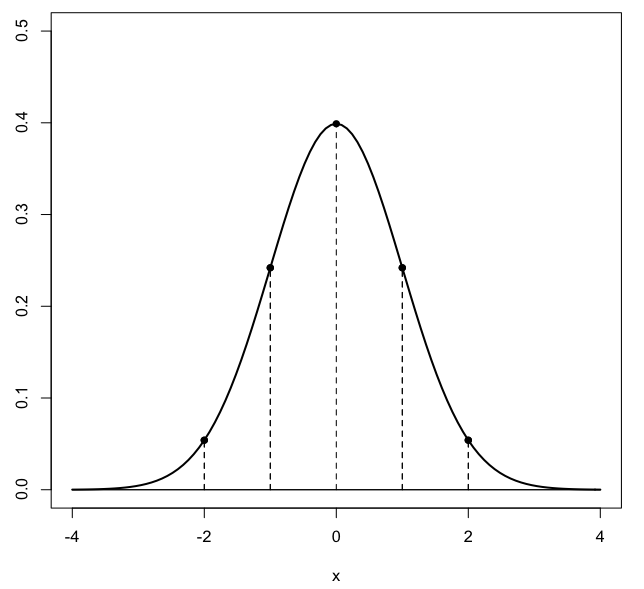
\includegraphics [scale=0.4] {gauss3.png} \end{center}

\title{Volume of a pyramid}
\date{}

\begin{document}
\maketitle
\Large

We need a formula for the volume of a cone in order to find the volume of a sphere.

Let's start with something simpler, a pyramid with a square base.  Consider a cube with all eight edges having length $s$.  So each of the six faces is a square with sides of length $s$ and area $s^2$.

Label the central point inside the solid as $P$.  Draw lines connecting each of the 8 external vertices to $P$, something like this. 
\begin{center}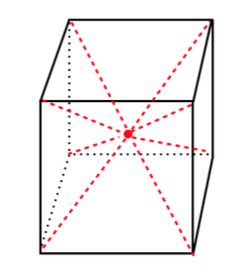
\includegraphics [scale=0.5] {cube_to_cone.png}\end{center}

Now we imagine slicing on planes that connect adjacent pairs of lines.  

You can't do this in real life by slicing up a single cube or rectangular solid, because the cuts to form one surface would ruin some of the other pieces.  The cuts must enter the solid at a corner and then pivot on a line ending at the exact center.  (Perhaps you could do it with a \emph{light saber} since the beam comes to a point).

The result is 6 identical pieces (square pyramids) looking something like this
\begin{center}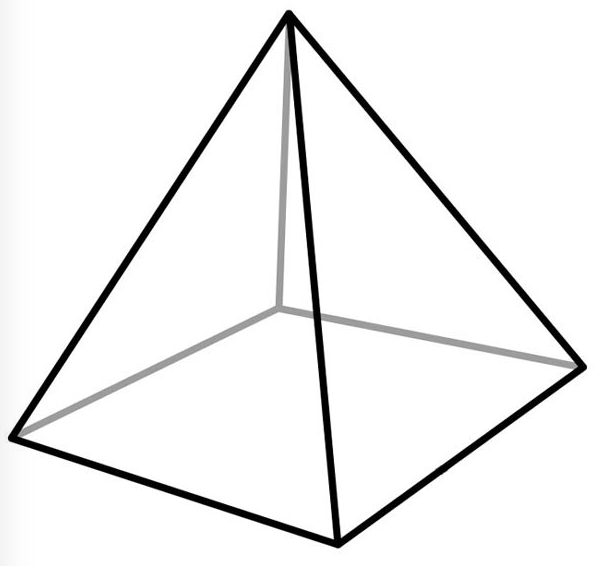
\includegraphics [scale=0.2] {squarepyramid.png}\end{center}

This figure isn't quite accurate because the procedure described above generates pyramids with height $s/2$.  They are a little squat, but just bear with me.

We started with a cube so that the six resulting solids would be identical.  Unfortunately you can either have six pieces the exactly the same, as we've done, or make it so some of the pieces come out with equal base and height, but you can't do both at the same time by this construction.

Let the six identical pyramid volumes each be $V$, and their sum is equal to the volume that we started with.  We have that
\[ 6V = s^3 \]
\[ V = \frac{1}{6} s^3  \]
This is the volume for each pyramid with base area $s^2$ and height $s/2$.  

The volume depends on both the area of the base and the height.  The more general formula for a pyramid is really a linear function of $h$
\[ V = \frac{1}{3} hs^2 \]

You can show this by starting with solids that are longer in one-dimension.  Since here $h = s/2$ it all works out.

Here is an even better way to slice a cube

\begin{center}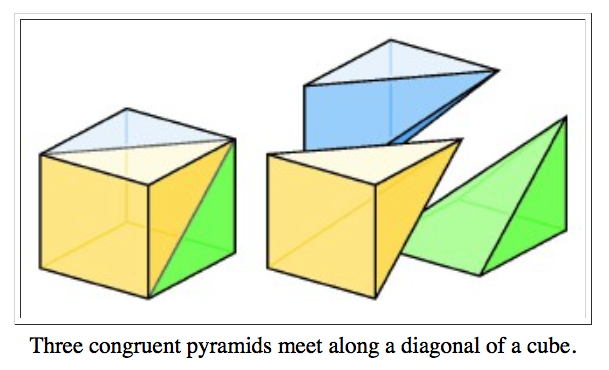
\includegraphics [scale=0.5] {pyramid_cube.png}\end{center}

When I first saw this, I thought it was a trick.  But in fact, we have produced $3$ identical right square pyramids.

\url{http://www.math.brown.edu/~banchoff/Beyond3d/chapter2/section02.html}

I know it sounds complicated but it's really not.

\subsection*{real world}

I found a fun way to do this demonstration easily.  Get a thick piece of cheese and cut out a cube as large as you can and as accurately as you can make it.  Then cut straight down on a diagonal all the way through that cube, resulting two identical pieces.

If you take these pieces and orient them correctly, you can make another diagonal cut straight down for each (left panel).  

\begin{center}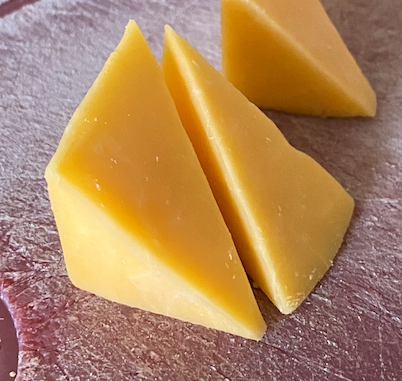
\includegraphics [scale=0.4] {cheese2.png}\end{center}

You end up with two large pieces and two small ones.  The two smaller ones can be assembled into a single shape identical with the large pieces.  

\begin{center}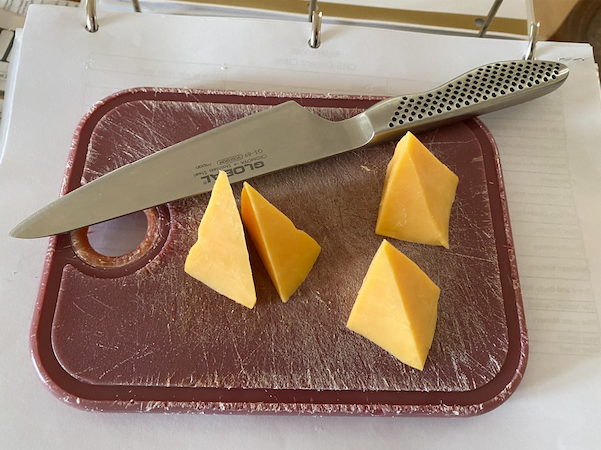
\includegraphics [scale=0.5] {cheese1.png}\end{center}

You have thus de-constructed the cube into three identical right pyramids.

Good luck!  You may eat the demonstration afterwards.

\subsection*{cones}

Of course, a pyramid is not a cone.  But an argument identical to the one we will use for the sphere shows that the volume is independent of the shape of the base.  It just depends on the area.  So for a cone we finally obtain
\[ V =  \frac{1}{3} \pi r^2 h \]

I found an algebraic derivation of the factor of one-third, that is given \hyperref[sec:one_third]{\textbf{here}}.

And we will revisit this problem, to employ our first useful bit of calculus.  Then we'll see that the factor of one-third arises naturally from the fact that the area of the base goes like the radius squared.

\end{document}